\documentclass[10pt]{article}

\usepackage[table,xcdraw]{xcolor}
\usepackage[utf8]{inputenc}
\usepackage{tabularx}
\usepackage{hyperref}
\usepackage{array}
\usepackage{graphicx} % Per inserire immagini (loghi)
\usepackage{geometry} % Per personalizzare i margini
\usepackage{fancyhdr} % Per gestire intestazioni e piè di pagina
\usepackage{tikz}
\usepackage{ragged2e}
\usepackage{anyfontsize}
\usepackage{tabularx, etoolbox}
\usepackage{eso-pic} % Per aggiungere elementi grafici su tutte le pagine
\usepackage{float}
\usepackage{longtable}

\newcommand\version{1.0.0} %aggiunta versione come variabile

\graphicspath{{images/}}
%\graphicspath{{../images/}}

\setcounter{secnumdepth}{4}
\setcounter{tocdepth}{4}

%cambio misure della pagina
\geometry{a4paper,left=25mm,right=25mm,top=25mm,bottom=25mm}
\definecolor{colorePie}{HTML}{ebdfc7}
\pagestyle{fancy}
\fancyhf{}
\renewcommand{\headrulewidth}{0.4pt}
\lhead{
    \parbox[c]{1cm}{\includegraphics[width=1.1cm]{Sevenbitslogo.png}}
}
\rhead{\textcolor[HTML]{9e978a}{ PIANO DI QUALIFICA v\version}
}
\setlength{\headheight}{25pt}
\cfoot{\thepage}

\renewcommand*\contentsname{Indice}
\renewcommand{\listfigurename}{Elenco delle figure}
\renewcommand{\listtablename}{Elenco delle tabelle}

\begin{document}

% Pagina del titolo
\begin{titlepage}
    \setcounter{page}{0}
    \centering
    % Inserisci il logo del gruppo (modifica il percorso dell'immagine)
    \includegraphics[width=7.2cm]{Sevenbitslogo.png} \\[2cm]

    % Titolo
     {\fontsize{40}{40}\bfseries Piano di Qualifica}\selectfont \\[3.9em]

    % Sottotitolo
    {\huge NearYou\\ \vspace{3mm }Smart custom advertising platform} \\[2.7em]

    % Email del gruppo
    {\large sevenbits.swe.unipd@gmail.com} \\[3em]

    % Spazio per il logo dell'università
    \hfill

    \AddToShipoutPictureBG{ % Imposta il triangolo con logo
        \ifnum\value{page}=0
        \begin{tikzpicture}[overlay]

            % Definisce un triangolo blu in basso a destra
            \fill[colorePie]
                (current page.south east) -- ++(-9cm,0) -- ++(9cm,9cm);

            % Inserisce il logo all'interno del triangolo
            \node[anchor=south east, xshift=-0.3cm, yshift=0.3cm] at (current page.south east) {
                \includegraphics[width=4.5cm]{LogoUnipd.png}
            };
        \end{tikzpicture}
        \fi
    }

\vfill % Aggiunge spazio verticale per centrare il contenuto
\end{titlepage}
\newpage
\clearpage
\setcounter{page}{1}

% Registro Modifiche
\begin{center}
 \textbf{Registro modifiche}\\   
\end{center}

\renewcommand{\arraystretch}{1.5}
\rowcolors{0}{gray!11}{white} % Aggiunge colore alternato alle righe

\begin{longtable}{|>{\centering\arraybackslash}m{1.5cm}|>{\centering\arraybackslash}m{2cm}|>{\centering\arraybackslash}m{2.5cm}|>{\centering\arraybackslash}m{2.5cm}|>{\centering\arraybackslash}m{5cm}|}
\hline
\textbf{Versione} & \textbf{Data} & \textbf{Autore} & \textbf{Verificatore} & \textbf{Descrizione}\\
\endhead
    \hline
    1.0.0 & 2025-02-21 & Giovanni Cristellon & Leonardo Trolese & Approvazione documento per RTB$_G$\\
    \hline
    0.4.8 & 2025-02-21 & Trolese Leonardo & Manuel Gusella & Correzione errori minori\\
    \hline
    0.4.7 & 2025-02-18 & Trolese Leonardo & Pivetta Federico & Aggiunta ulteriori grafici sulle metriche del \hyperref[sec:cruscotto]{cruscotto di valutazione}\\
    \hline
    0.4.6 & 2025-02-16 & Trolese Leonardo & Pivetta Federico & Aggiunta ulteriori grafici sulle metriche del \hyperref[sec:cruscotto]{cruscotto di valutazione}\\
    \hline
    0.4.5 & 2025-02-15 & Trolese Leonardo & Pivetta Federico & Aggiunta grafici sulle metriche del \hyperref[sec:cruscotto]{cruscotto di valutazione}\\ 
    \hline
    0.4.4 & 2025-02-11 & Federico Pivetta & Uncas Peruzzi & Correzione ai test$_G$ di sistema$_G$ e di accettazione a seguito delle modifiche all'Analisi dei Requisiti\\
    \hline
    0.4.3 & 2025-01-14 & Federico Pivetta & Leonardo Trolese & Riorganizzazione delle metriche di qualità\\
    %\hline
    %0.4.3 & 2025-01-10 & Leonardo Trolese & Uncas Peruzzi & Aggiunta dei test$_G$ di integrazione\\
    \hline
    0.4.2 & 2025-01-10 & Federico Pivetta & Leonardo Trolese & Aggiunta dei test$_G$ di sistema$_G$ e dei test$_G$ di accettazione\\
    \hline
    0.4.1 & 2025-01-08 & Riccardo Piva & Uncas Peruzzi & Refactor generale sezione qualità processo$_G$ e qualità prodotto \\
    \hline
    0.4.0 & 2025-01-07 & Riccardo Piva & Uncas Peruzzi & Creazione cruscotto$_G$\\
    \hline
    0.3.3 & 2025-01-03 & Riccardo Piva & Uncas Peruzzi & Correzioni minori generali \\
    \hline
    0.3.2 & 2024-12-16 & Alfredo Rubino & Manuel Gusella & Aggiunta acronimi metriche e correzioni minori\\
    \hline
    0.3.1 & 2024-12-13 & Riccardo Piva & Alfredo Rubino & Correzione standard IEEE$_G$ \\
    \hline
    0.3.0 & 2024-12-12 & Riccardo Piva & Alfredo Rubino & Arricchimento sezioni Qualità di processo$_G$, Qualità di prodotto e inizio redazione modalità testing \\
    \hline
    0.2.0 & 2024-12-06 & Manuel Gusella  & Alfredo Rubino & Inizio redazione sottosezione Qualità di prodotto\\
    \hline
    0.1.0 & 2024-11-21 & Uncas Peruzzi  & Federico Pivetta & Inizio redazione del documento\\
    \hline
\end{longtable}
\rowcolors{0}{}{} % Riporta le righe alla colorazione originale

\newpage
\tableofcontents
\newpage
\listoffigures %elenco delle figure sarà da usare per ogni immagine
\newpage
\listoftables %lista delle tabelle presenti nel documento
\newpage
\begin{justify}

\section{Introduzione}

\subsection{Scopo del documento}
Il seguente documento ha l'obiettivo di garantire la qualità del prodotto e dei processi coinvolti nell'intero progetto$_G$. Al fine di assicurare che il prodotto soddisfi le aspettative di qualità attese, il documento
verrà aggiornato nel tempo per riflettere eventuali modifiche, integrazioni e i risultati delle verifiche effettuate.


\subsection{Glossario}
Con l'intento di evitare ambiguità nell'interpretazione del linguaggio utilizzato, viene fornito un glossario che si occupa di esplicitare il significato dei termini che riguardano il contesto del progetto$_G$. I termini presenti nel glossario sono contrassegnati con una $_G$ a pedice : Termine$_G$.\\
Le definizioni sono contenute nell'apposito documento \textit{Glossario}.\\


\subsection{Riferimenti}


\subsubsection{Riferimenti normativi}
\begin{itemize}
    \item[-] \textit{Norme\_di\_Progetto\_v1.0.0}

    \item[-] Regolamento del progetto$_G$ didattico  \\
      \textcolor{blue}{\texttt{\url{https://www.math.unipd.it/~tullio/IS-1/2024/Dispense/PD1.pdf}}}\\
      (Consultato: 2025-02-19).
    \item[-] Capitolato$_G$ C4 - NearYou - Smart custom advertising platform\\
    \textcolor{blue}{\texttt{\url{https://www.math.unipd.it/~tullio/IS-1/2024/Progetto/C4p.pdf}}}\\
    (Consultato: 2025-02-19).\\
    \textcolor{blue}{\texttt{\url{https://www.math.unipd.it/~tullio/IS-1/2024/Progetto/C4.pdf}}}\\
    (Consultato: 2025-02-19).
    
    \item[-] Standard ISO/IEC 9126 \label{ISO 9126} \\
    \textcolor{blue}{\texttt{\url{https://en.wikipedia.org/wiki/ISO/IEC_9126}}}\\
    (Consultato: 2025-02-19).
    \item[-] Standard ISO/IEC/IEEE 12207:1995 \label{ISO 12207:1995}\\
    \textcolor{blue}{\texttt{\url{https://www.math.unipd.it/~tullio/IS-1/2009/Approfondimenti/ISO_12207-1995.pdf}}}\\
    (Consultato: 2025-02-19).

\end{itemize}
\subsubsection{Riferimenti informativi}
\begin{itemize}
    \item[-] Qualità di prodotto\\
    \textcolor{blue}{\texttt{\url{https://www.math.unipd.it/~tullio/IS-1/2024/Dispense/T07.pdf}}}\\
    (Consultato: 2025-02-19).
    \item[-] Qualità di processo$_G$\\
    \textcolor{blue}{\texttt{\url{https://www.math.unipd.it/~tullio/IS-1/2024/Dispense/T08.pdf}}}\\
    (Consultato: 2025-02-19).
    \item[-] Verifica e validazione\\
    \textcolor{blue}{\texttt{\url{https://www.math.unipd.it/~tullio/IS-1/2024/Dispense/T09.pdf}}}\\
    (Consultato: 2025-02-19).\\
    \textcolor{blue}{\texttt{\url{https://www.math.unipd.it/~tullio/IS-1/2024/Dispense/T10.pdf}}}\\
    (Consultato: 2025-02-19).\\
    \textcolor{blue}{\texttt{\url{https://www.math.unipd.it/~tullio/IS-1/2024/Dispense/T11.pdf}}}\\
    (Consultato: 2025-02-19).
\end{itemize}
\newpage

\section{Obiettivi metrici di qualità}
Per far sì che un prodotto raggiunga uno standard qualitativo, è necessario definire delle metriche precise che permettano di monitorare e indicare il grado di qualità del prodotto e che quindi permettano di definire questo standard.
Queste metriche vengono definite nel documento \textit{Norme di Progetto$_G$}.
Questa sezione si occuperà di definire i parametri di accettazione e ottimalità delle relative metriche.\\

\subsection{Qualità di prodotto}
La qualità di prodotto è intesa come valutazione del software, e più precisamente per la determinazione del grado di conformità alle attese.\\
Si rivolge l'attenzione su aspetti come Usabilità, Affidabilità e Manutenibilità, ma più in generale alla qualità esterna (funzionale) ed interna (strutturale) del prodotto software.\\
Quindi non basta che il software implementi le funzionalità richieste dal proponente$_G$, ma le esegua secondo specifici standard di qualità.\\
In seguito sono presenti le metriche definite dallo \hyperref[ISO 9126]{standard ISO/IEC 9126} che il gruppo si impegna a soddisfare per la qualità del prodotto software.
\subsubsection{Funzionalità}
\begin{table}[H]
  \centering
\begin{tabular}{|c|c|c|c|}
  \hline
  \textbf{Metrica} & \textbf{Descrizione} & \textbf{Valore accettazione} & \textbf{Valore ideale}\\
  \hline
  MPD01 & Requisiti Obbligatori Soddisfatti & 100\% & 100\%\\
  \hline
  MPD02 & Requisiti Desiderabili Soddisfatti  & $\geq$ 0\% & 100\% \\
  \hline
  MPD03 & Requisiti Opzionali Soddisfatti & $\geq$ 0\% & 100\% \\
  \hline
  MPD04 & Function Point & da determinare & da determinare \\ 
  \hline
\end{tabular}
\caption{Funzionalità - Qualità di prodotto}
\label{tab:funzionalità}
\end{table}

\subsubsection{Affidabilità}
\begin{table}[H]
  \centering
\begin{tabular}{|c|c|c|c|}
  \hline
  \textbf{Metrica} & \textbf{Descrizione} & \textbf{Valore accettazione} & \textbf{Valore ideale}\\
  \hline
  MPD05 & Code coverage & $\geq$ 80\% & 100\% \\
  \hline
  MPD06 & Statement coverage & $\geq$ 80\% & 100\% \\
  \hline
  MPD07 & Branch$_G$ coverage & $\geq$ 80\% & 100\% \\
  \hline
  MPD08 & Condition coverage & $\geq$ 80\% & 100\% \\
  \hline
\end{tabular}
\caption{Affidabilità - Qualità di prodotto}
\label{tab:affidabilità}
\end{table}

\subsubsection{Efficienza}
\begin{table}[H]
  \centering
\begin{tabular}{|c|c|c|c|}
  \hline
  \textbf{Metrica} & \textbf{Descrizione} & \textbf{Valore accettazione} & \textbf{Valore ideale}\\
  \hline
  MPD09 & Tempo medio di risposta & $\leq$ 10 secondi & $\leq$ 4 secondi \\
  \hline
\end{tabular}
\caption{Efficienza - Qualità di prodotto}
\label{tab:efficienza}
\end{table}

\subsubsection{Usabilità}
\begin{table}[H]
  \centering
\begin{tabular}{|c|c|c|c|}
  \hline
  \textbf{Metrica} & \textbf{Descrizione} & \textbf{Valore accettazione} & \textbf{Valore ideale}\\
  \hline
  MPD10 & Facilità di utilizzo & $\leq$ 7 click & $\leq$ 5 click\\
  \hline
  MPD11 & Tempo medio di apprendimento & $\leq$ 5 minuti & $\leq$ 2 minuti \\
  \hline
\end{tabular}
\caption{Usabilità - Qualità di prodotto}
\label{tab:usabilità}
\end{table}

\subsubsection{Manutenibilità}
\begin{table}[H]
  \centering
\begin{tabular}{|c|c|c|c|}
  \hline
  \textbf{Metrica} & \textbf{Descrizione} & \textbf{Valore accettazione} & \textbf{Valore ideale}\\
  \hline
  MPD12 & Coefficiente di accoppiamento fra classi & $\leq$ 4 & $\leq$ 2 \\
  \hline
  MPD13 & Linee di codice per metodo & $\leq$ 50 & $\leq$ 25 \\
  \hline
  MPD14 & Parametri per metodo & $\leq$ 7 & $\leq$ 4 \\
  \hline
  MPD15 & Attributi per classe & $\leq$ 7 & $\leq$ 5 \\
  \hline
  MPD16 & Structure Fan IN & - & va massimizzato \\
  \hline
  MPD17 & Structure Fan OUT & - & va minimizzato \\
  \hline
\end{tabular}
\caption{Manutenibilità - Qualità di prodotto}
\label{tab:manutenibilità}
\end{table}

\subsubsection{Portabilità}
\begin{table}[H]
  \centering
\begin{tabular}{|c|c|c|c|}
  \hline
  \textbf{Metrica} & \textbf{Descrizione} & \textbf{Valore accettazione} & \textbf{Valore ideale}\\
  \hline
  MPD18 & Versioni browser supportati & $\geq$ 80\% & 100\% \\
  \hline
\end{tabular}
\caption{Portabilità - Qualità di prodotto}
\label{tab:portabilità}
\end{table}


\subsection{Qualità di processo$_G$}
La qualità di processo$_G$ è intesa come valutazione delle attività svolte per la realizzazione del prodotto.\\
Seguendo delle buone pratiche e delle linee guida nello sviluppo software, si può garantire che il prodotto finale avrà rispettato a sua volta degli standard qualitativi rendendolo così un prodotto di qualità.\\
Qui sotto divideremo le metriche di qualità di processo$_G$ seguendo lo \hyperref[ISO 12207:1995]{standard ISO/IEC 12207:1995} in tre categorie: Processi primari, Processi di supporto e Processi organizzativi.\\
\subsubsection{Processi Primari}
I processi primari si possono dividere in parti primarie e una parte primaria è quella che inizia o esegue lo sviluppo, l'operazione o la manutenzione di prodotti software.\\

\paragraph{Fornitura}\mbox{}\\
La fornitura è il processo$_G$ che si occupa di consegnare il prodotto software al cliente.\\
Serve per garantire che il prodotto soddisfi i requisiti di tempi e costi definiti con il cliente.\\
\begin{table}[H]
\centering
\begin{tabular}{|>{\centering\arraybackslash}p{1.5cm}|>{\centering\arraybackslash}p{5cm}|>{\centering\arraybackslash}p{4cm}|>{\centering\arraybackslash}p{3.7cm}|}
  \hline
  \textbf{Metrica} & \textbf{Descrizione} & \textbf{Valore accettazione} & \textbf{Valore ideale}\\
  \hline
  MPC01 & Estimated at completion (EAC) & \textpm5\% rispetto al (BAC)\(_G\) & Budget at completion (BAC)\(_G\)\\
  \hline
  MPC02 & Estimate to complete (ETC) & $\geq$ 0 & $\leq$ EAC$_G$\(_G\) \\
  \hline
  MPC03 & Actual cost (AC) & $\geq$ 0 & $\leq$ EAC$_G$\(_G\) \\
  \hline
  MPC04 & Earned value (EV) & $\geq$ 0 & $\leq$ EAC$_G$\(_G\) \\
  \hline
  MPC05 & Planned value (PV) & $\geq$ 0 & $\leq$ Budget at completion (BAC)\(_G\) \\
  \hline
  MPC06 & Schedule variance (SV) & $\geq$ -5\% rispetto al (BAC)\(_G\) & $\geq$ 0\% \\
  \hline
  MPC07 & Cost variance (CV) & $\geq$ -5\% rispetto al (BAC)\(_G\) & $\geq$ 0\% \\
  \hline
  MPC08 & Cost Performance Index (CPI) & $\geq$ 0.9 & $\geq$ 1.0 \\
  \hline
\end{tabular}
\caption{Processi primari - Fornitura}
\label{tab:fornitura}
\end{table}

\paragraph{Sviluppo}\mbox{}\\
Lo sviluppo è il processo$_G$ riguardante la scrittura del codice del prodotto software.\\
Questa metrica serve a garantire che il software rispetti le richieste del cliente e che la codifica avvenga in modo efficiente\\
\begin{table}[H]
  \centering
\begin{tabular}{|c|c|c|c|}
  \hline
  \textbf{Metrica} & \textbf{Descrizione} & \textbf{Valore accettazione} & \textbf{Valore ideale}\\
  \hline
  MPC09 & Requisiti Obbligatori Soddisfatti (ROS) & 100\% & 100\%\\
  \hline
  MPC10 & Requirements Stability Index (RSI) & $\geq$ 80\% & 100\% \\
  \hline
\end{tabular}
\caption{Processi primari - Codifica}
\label{tab:codifica}
\end{table}


\subsubsection{Processi di Supporto}
Un processo$_G$ di supporto è un processo$_G$ che supporta un altro processo$_G$ come parte integrante con uno scopo distinto e contribuisce al successo e alla qualità del progetto$_G$ software.\\
Un processo$_G$ di supporto è impiegato ed eseguito, se necessario, da un altro processo$_G$.\\
\paragraph{Documentazione}\mbox{}\\
La documentazione$_G$ è essenziale per la comprensione del prodotto e per la sua manutenzione.\\
Di conseguenza è essenziale che questa sia chiara, comprensibile e corretta.\\
\begin{table}[H]
  \centering
\begin{tabular}{|c|c|c|c|}
  \hline
  \textbf{Metrica} & \textbf{Descrizione} & \textbf{Valore accettazione} & \textbf{Valore ideale}\\
  \hline
  MPC11 & Indice Gulpease & $\geq$ 40\% & $\geq$ 60\% \\
  \hline
  MPC12 & Correttezza ortografica & 0 errori & 0 errori \\
  \hline
\end{tabular}
\caption{Processi di supporto - Documentazione$_G$}
\label{tab:documentazione}
\end{table}

\paragraph{Verifica}\mbox{}\\
La verifica serve a garantire che il prodotto software sia conforme alle specifiche e non contenga errori.\\
\begin{table}[H]
  \centering
\begin{tabular}{|c|c|c|c|}
  \hline
  \textbf{Metrica} & \textbf{Descrizione} & \textbf{Valore accettazione} & \textbf{Valore ideale}\\
  \hline
  MPC13 & Code coverage & $\geq$ 80\% & 100\% \\
  \hline
  MPC14 & Passed test$_G$ cases percentage & $\geq$ 80\% & 100\% \\
  \hline
\end{tabular}
\caption{Processi di supporto - Verifica}
\label{tab:verifica}
\end{table}

\paragraph{Gestione della qualità}\mbox{}\\
La gestione della qualità è necessaria per garantire che tutte le metriche di qualità vengano effettivamente soddisfatte.\\
\begin{table}[H]
  \centering
\begin{tabular}{|c|c|c|c|}
  \hline
  \textbf{Metrica} & \textbf{Descrizione} & \textbf{Valore accettazione} & \textbf{Valore ideale}\\
  \hline
  MPC15 & Metriche di qualità soddisfate & $\geq$ 85\% & 100\% \\
  \hline
\end{tabular}
\caption{Processi di supporto - Gestione della qualità}
\label{tab:gestione della qualità}
\end{table}

\subsubsection{Processi Organizzativi}
I processi organizzativi servono per creare un sottostruttura per il ciclo-di-vita$_G$ e
per garantire che i processi principali e i loro processi di supporto siano ben strutturati e vengano continuamente migliorati.\\
\paragraph{Gestione dei processi}\mbox{}\\
La gestione dei processi indica come vengono gestiti i processi all'interno del progetto$_G$.\\
\begin{table}[H]
  \centering
\begin{tabular}{|c|c|c|c|}
  \hline
  \textbf{Metrica} & \textbf{Descrizione} & \textbf{Valore accettazione} & \textbf{Valore ideale}\\
  \hline
  MPC16 & Rischi non previsti & $\leq$ 3 & 0 \\
  \hline
  MPC17 & Efficienza$_G$ temporale (ET) & $\geq$ 0.2 & $\geq$ 1.0 \\
  \hline
\end{tabular}
\caption{Processi organizzativi - Gestione dei processi}
\label{tab:gestione dei processi}
\end{table}
\newpage

\section{Modalità di Testing}
Qui sotto sono elencati i vari test$_G$ che vengono eseguiti automaticamente sul prodotto software.\\
Questo serve a garantire che il prodotto soddisfi i requisiti e le aspettative indicate nel documento \textit{Analisi dei Requisiti}.\\
I test$_G$ sono divisi in quattro categorie: Test$_G$ di unità, Test$_G$ di sistema$_G$, Test$_G$ di integrazione e Test$_G$ di accettazione.\\
E per indicare lo stato come indicato in \textit{Norme di Progetto$_G$} vengono utilizzate le seguenti abbreviazioni:
\begin{itemize}
\item \textbf{P}: Passato
\item \textbf{NP}: Non Passato
\item \textbf{NI}: Non Implementato
\end{itemize}

\subsection{Test di unità}
I test$_G$ di unità servono a verificare che ogni singola unità del software funzioni correttamente.\\

\subsection{Test di sistema$_G$}
I test$_G$ di sistema$_G$ servono a verificare la completa copertura dei requisiti concordati nel documento \textit{Analisi dei Requisiti}.\\

\begin{longtable}{|>{\centering\arraybackslash}m{2cm}|>{\centering\arraybackslash}m{7cm}|>{\centering\arraybackslash}m{2cm}|>{\centering\arraybackslash}m{2cm}|}
\hline
\textbf{Codice} & \textbf{Descrizione} & \textbf{Requisito} & \textbf{Stato}\\
\endhead
\hline
TS1 & Verificare che l'utente privilegiato possa visualizzare la Dashboard$_G$ composta da una mappa interattiva con i vari Marker$_G$ su di essa. & RF01 & NI \\
\hline
TS2 & Verificare che l'utente privilegiato possa visualizzare dei Marker$_G$ che rappresentano i vari Percorsi$_G$ effettuati in tempo reale dagli utenti presenti nel Sistema$_G$ & RF02 & NI \\
\hline
TS3 & Verificare che l'utente privilegiato possa visualizzare un Marker$_G$ che rappresenta un Percorso$_G$ effettuato in tempo reale da un utente presente nel Sistema$_G$ & RF03 & NI \\
\hline
TS4 & Verificare che l'utente privilegiato possa visualizzare tutti i punti di interesse riconosciuti dal Sistema$_G$. & RF04 & NI \\
\hline
TS5 & Verificare che l'utente privilegiato possa visualizzare un Marker$_G$ che rappresenta un punto di interesse riconosciuto dal Sistema$_G$. & RF05 & NI \\
\hline
TS6 & Verificare che l'utente privilegiato possa visualizzare gli annunci pubblicitari provenienti da un determinato punto di interesse. & RF06 & NI \\
\hline
TS7 & Verificare che l'utente privilegiato possa visualizzare un singolo annuncio pubblicitario tramite un Marker$_G$. & RF07 & NI \\
\hline
TS8 & Verificare che l'utente privilegiato possa visualizzare una Dashboard$_G$ relativa ad un singolo utente quando seleziona un Marker$_G$ utente nella Dashboard$_G$ principale. & RF08 & NI \\
\hline
TS9 & Verificare che l'utente privilegiato possa visualizzare dei Marker$_G$ che rappresentano lo storico delle posizioni dell'utente a cui è riferita la Dashboard$_G$ di singolo utente. & RF09 & NI \\
\hline
TS10 & Verificare che l'utente privilegiato possa visualizzare un Marker$_G$ che rappresenta la posizione dell'utente in un determinato istante nella Dashboard$_G$ di singolo utente. & RF10 & NI \\
\hline
TS11 & Verificare che l'utente privilegiato possa visualizzare, nella Dashboard$_G$ di singolo utente, tutti i punti di interesse riconosciuti dal Sistema$_G$. & RF11 & NI \\
\hline
TS12 & Verificare che l'utente privilegiato possa visualizzare, nella Dashboard$_G$ di singolo utente, un Marker$_G$ che rappresenta un punto di interesse riconosciuto dal Sistema$_G$. & RF12 & NI \\
\hline
TS13 & Verificare che l'utente privilegiato possa visualizzare lo storico degli annunci pubblicitari generati per l'utente a cui è riferita la Dashboard$_G$ singolo utente. & RF13 & NI \\
\hline
TS14 & Verificare che l'utente privilegiato possa visualizzare un singolo annuncio pubblicitario tramite un Marker$_G$ nella Dashboard$_G$ di singolo utente. & RF14 & NI \\
\hline
TS15 & Verificare che l'utente privilegiato possa visualizzare un pannello apposito contenente le informazioni dell'utente, a cui è riferita la Dashboard$_G$ di singolo utente, in forma tabellare. & RF15 & NI \\
\hline
TS16 & Verificare che l'utente privilegiato possa visualizzare nel pannello apposito di visualizzazione informazioni dell'utente: il nome, il cognome, l'email, il genere, la data di nascita e lo stato civile. & RF16 & NI \\
\hline
TS17 & Verificare che l'utente privilegiato possa visualizzare i dettagli del Marker$_G$ riguardante una singola posizione di un utente nella rispettiva Dashboard$_G$ & RF17 & NI \\
\hline
TS18 & Verificare che l'utente privilegiato quando visualizza i dettagli del Marker$_G$, riguardante una singola posizione di un utente nella rispettiva Dashboard$_G$, possa vedere la latitudine, la longitudine e l'istante di rilevamento del Marker$_G$ & RF18 & NI \\
\hline
TS19 & Verificare che l'utente privilegiato possa visualizzare l'area di influenza di un punto di interesse selezionato. & RF19 & NI \\
\hline
TS20 & Verificare che l'utente privilegiato possa visualizzare le informazioni dettagliate di un punto di interesse quando selezionato. & RF20 & NI \\
\hline
TS21 & Verificare che l'utente privilegiato quando visualizza le informazioni dettagliate di un punto di interesse possa visualizzare la latitudine, la longitudine, il nome, la tipologia e la descrizione del punto di interesse. & RF21 & NI \\
\hline
TS22 & Verificare che l'utente possa visualizzare l'annuncio pubblicitario proveniente dal punto di interesse situato nell'area che sta attraversando. & RF22 & NI \\
\hline
TS23 & Verificare che l'utente privilegiato possa visualizzare una tabella contenente le informazioni dei singoli PoI ordinati per la quantità di messaggi inviati nel mese. & RF23 & NI \\
\hline
TS24 & Verificare che l'utente privilegiato possa visualizzare nella tabella dei PoI un singolo PoI, rappresentato da una riga della tabella. & RF24 & NI \\
\hline
TS25 & Verificare che l'utente privilegiato possa visualizzare in ogni riga della tabella dei PoI il nome, l'indirizzo, la tipologia (di che ambito si occupa), la descrizione e il numero di messaggi inviati durante il mese di un singolo PoI. & RF25 & NI \\
\hline
TS26 & Verificare che l'utente privilegiato possa visualizzare i dettagli di un annuncio generato. & RF26 & NI \\
\hline
TS27 & Verificare che l'utente privilegiato quando visualizza i dettagli di un annuncio possa visualizzare la latitudine, la longitudine, l'istante di creazione, il nome dell'utente coinvolto, il nome del punto di interesse coinvolto e il contenuto dell'annuncio. & RF27 & NI \\
\hline
TS28 & Verificare che il sensore possa trasmettere i dati rilevati in tempo reale al Sistema$_G$. & RF28 & NI\\
\hline
TS29 & Verificare che il sensore possa trasmettere il proprio id, la sua latitudine e longitudine al Sistema$_G$. & RF29 & NI\\
\hline
TS30 & Verificare che il servizio LLM$_G$ possa ricevere i dati dell'utente e del punto di interesse inviati dal Sistema$_G$. & RF30 & NI \\
\hline
TS31 & Verificare che il servizio LLM$_G$ possa ricevere le informazioni dell'utente inviate dal Sistema$_G$, quali: il nome, il cognome, l'email, il genere, la data di nascita, lo stato civile e i suoi interessi. & RF31 & NI \\
\hline
TS32 & Verificare che il servizio LLM$_G$ possa ricevere le informazioni del punto di interesse inviate dal Sistema$_G$, quali: il nome, l'indirizzo, la tipologia, la descrizione e la distanza del PoI dall'utente. & RF32 & NI \\
\hline
TS33 & Verificare che il servizio LLM$_G$ possa trasmettere un messaggio custom, rappresentante il contenuto dell'annuncio per un utente, al Sistema$_G$. & RF33 & NI \\
\hline
\caption{Test di sistema$_G$}\\
\end{longtable}

\subsection{Test di integrazione}
I test$_G$ di integrazione servono a verificare che le componenti del sistema$_G$ si integrino correttamente e in maniera efficace. L'obiettivo dei test$_G$
è identificare eventuali problemi di interoperabilità e integrazione fra le componenti del software.\\

%\begin{longtable}{|>{\centering\arraybackslash}m{2cm}|>{\centering\arraybackslash}m{7cm}|>{\centering\arraybackslash}m{2cm}|}
%\hline
%\textbf{Codice} & \textbf{Descrizione} & \textbf{Stato}\\
%\endhead
%\hline
%TI1 & Verificare che i dati simulati vengano correttamente pubblicati sul broker di messaggi & NI\\
%\hline
%TI2 & Assicurarsi che il modulo di stream processing elabori correttamente i dati ricevuti dal broker e li invii al motore di generative AI & NI\\
%\hline
%TI3 & Verificare che il motore LLM$_G$ generi messaggi pubblicitari coerenti e contestualizzati in base ai dati forniti & NI\\
%\hline
%TI4 & Controllare che i messaggi generati vengano correttamente salvati nella piattaforma di storage & NI\\
%\hline
%TI5 & Controllare che i dati posizionali generati vengano correttamente salvati nella piattaforma di storage & NI\\
%\hline
%TI6 & Verificare che i dati geospaziali vengano aggiornati in tempo reale sulla dashboard$_G$ contenente la mappa & NI\\
%\hline
%TI7 & Assicurarsi che i messaggi generati dal motore LLM$_G$ siano correttamente visualizzati nella dashboard$_G$ & NI\\
%\hline
%\caption{Test di integrazione}\\
%\end{longtable}

\subsection{Test di accettazione}
I test$_G$ di accettazione sono finalizzati a verificare che tutte le esigenze concordate con il proponente$_G$ siano soddisfatte, e di conseguenza saranno
svolti al termine del progetto$_G$ dai membri del gruppo in coordinazione con i componenti dell'azienda Synclab$_G$.\\

\begin{longtable}{|>{\centering\arraybackslash}m{2cm}|>{\centering\arraybackslash}m{7cm}|>{\centering\arraybackslash}m{2cm}|}
\hline
\textbf{Codice} & \textbf{Descrizione} & \textbf{Stato}\\
\endhead
\hline
TA1 & Verificare che l'utente privilegiato possa visualizzare la Dashboard$_G$ composta da una mappa e interagire con i Marker$_G$ presenti su di essa. & NI \\
\hline
TA2 & Verificare che l'utente privilegiato possa visualizzare sulla mappa tutti i Marker$_G$ relativi ai Percorsi effettuati in tempo reale dagli utenti, ai punti di interesse riconosciuti dal Sistema$_G$ e agli annunci pubblicitari associati ai punti di interesse. & NI \\
\hline
TA3 & Verificare che l'utente privilegiato possa visualizzare una Dashboard$_G$ relativa ad un singolo utente quando seleziona un Marker$_G$ utente nella Dashboard$_G$ principale & NI \\
\hline
TA4 & Verificare che l'utente privilegiato possa visualizzare, nella Dashboard$_G$ relativa ad un singolo utente, tutti i punti di interesse riconosciuti dal Sistema$_G$, lo storico delle posizioni dell'utente, lo storico degli annunci pubblicitari generati per l'utente, un pannello dedicato con le informazioni dell'utente in forma tabellare e i dettagli relativi a ciascuna posizione. & NI \\
\hline
TA5 & Verificare che l'utente privilegiato possa visualizzare, nella Dashboard$_G$ relativa a un singolo utente, i dettagli del pannello, inclusi il nome, il cognome, l'email, il genere, la data di nascita e lo stato civile. Inoltre, verificare che siano visibili i dettagli della singola posizione, inclusi la latitudine, la longitudine e l'istante di rilevamento. & NI \\
\hline
TA6 & Verificare che l'utente privilegiato possa visualizzare i dettagli di un punto di interesse, inclusi la latitudine, la longitudine, il nome, la tipologia e la descrizione. & NI \\
\hline
TA7 & Verificare che l'utente privilegiato possa visualizzare i dettagli di un annuncio generato, inclusi la latitudine, la longitudine, l'istante di creazione, il nome dell'utente coinvolto, il nome del punto di interesse coinvolto e il contenuto dell'annuncio. & NI \\
\hline
TA8 & Verificare che l'utente privilegiato possa visualizzare una tabella contenente l'elenco dei punti di interesse, ordinati per la quantità di messaggi inviati nel mese. Ogni PoI deve essere rappresentato da una riga della tabella, contenente il nome, l'indirizzo, la tipologia, la descrizione e il numero di messaggi inviati. & NI \\
\hline
TA9 & Verificare che il sensore possa trasmettere in tempo reale al Sistema$_G$ i dati rilevati, inclusi il proprio id, la latitudine e la longitudine. & NI \\
\hline
TA10 & Verificare che il servizio LLM$_G$ possa ricevere i dati inviati dal Sistema$_G$, inclusi le informazioni dell'utente (nome, cognome, email, genere, data di nascita, stato civile, interessi) e le informazioni del punto di interesse (nome, indirizzo, tipologia, descrizione e distanza dal punto di interesse dell'utente). & NI \\
\hline
TA11 & Verificare che il servizio LLM$_G$ possa trasmettere al Sistema$_G$ un messaggio personalizzato che rappresenti il contenuto dell'annuncio destinato ad un utente. & NI \\
\hline
\caption{Test di accettazione}\\
\end{longtable}


\section{Cruscotto di valutazione delle qualità}
\label{sec:cruscotto}
\subsection{Qualità di processo$_G$ - fornitura}
\label{sec:QdP_fornitura}
\subsubsection{MPC01 - Estimated at completion (EAC)}

\begin{figure}[H]
  \centering
  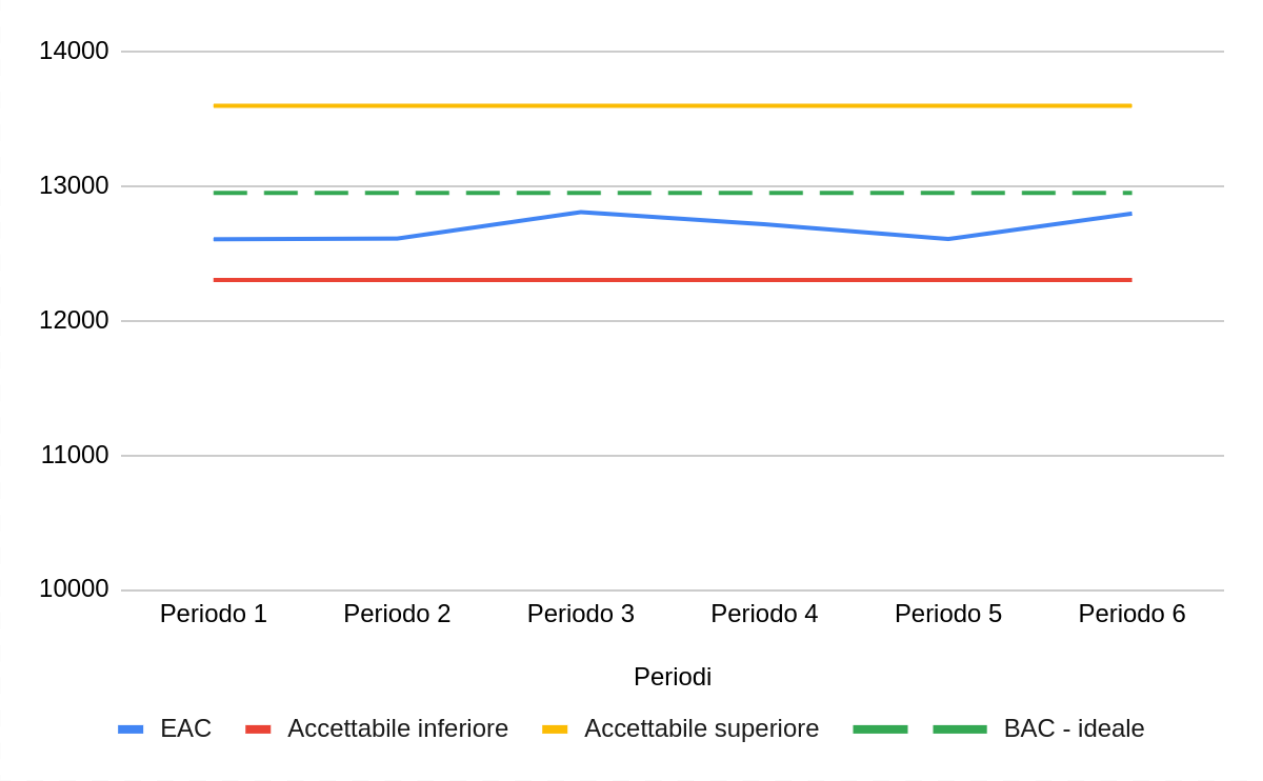
\includegraphics[width=0.9\linewidth]{EAC.png}
  \caption{Grafico a linee della metrica EAC$_G$}
  \label{fig:EACchart}
\end{figure}


\textbf{RTB}: Il grafico rappresenta la stima aggiornata del costo totale del progetto$_G$ al completamento. Questo valore è quindi determinato dalla somma 
dei costi sostenuti fino a un certo momento (in termini di ore produttive svolte), e dei costi stimati al completamento (in termini di ore produttive 
restanti in riferimento al preventivo iniziale del progetto$_G$).\\ 
In questo caso emerge dal grafico che il valore di EAC$_G$ è poco al di sotto del preventivo iniziale (BAC), e in ogni caso entro i valori accettabili definiti
per la metrica. Questo indica che il progetto$_G$ è sufficientemente in linea con le aspettative in termini di costi.


\subsubsection{MPC05 - Planned Value (PV) \& MPC04 - Earned Value (EV)}

\begin{figure}[H]
  \centering
  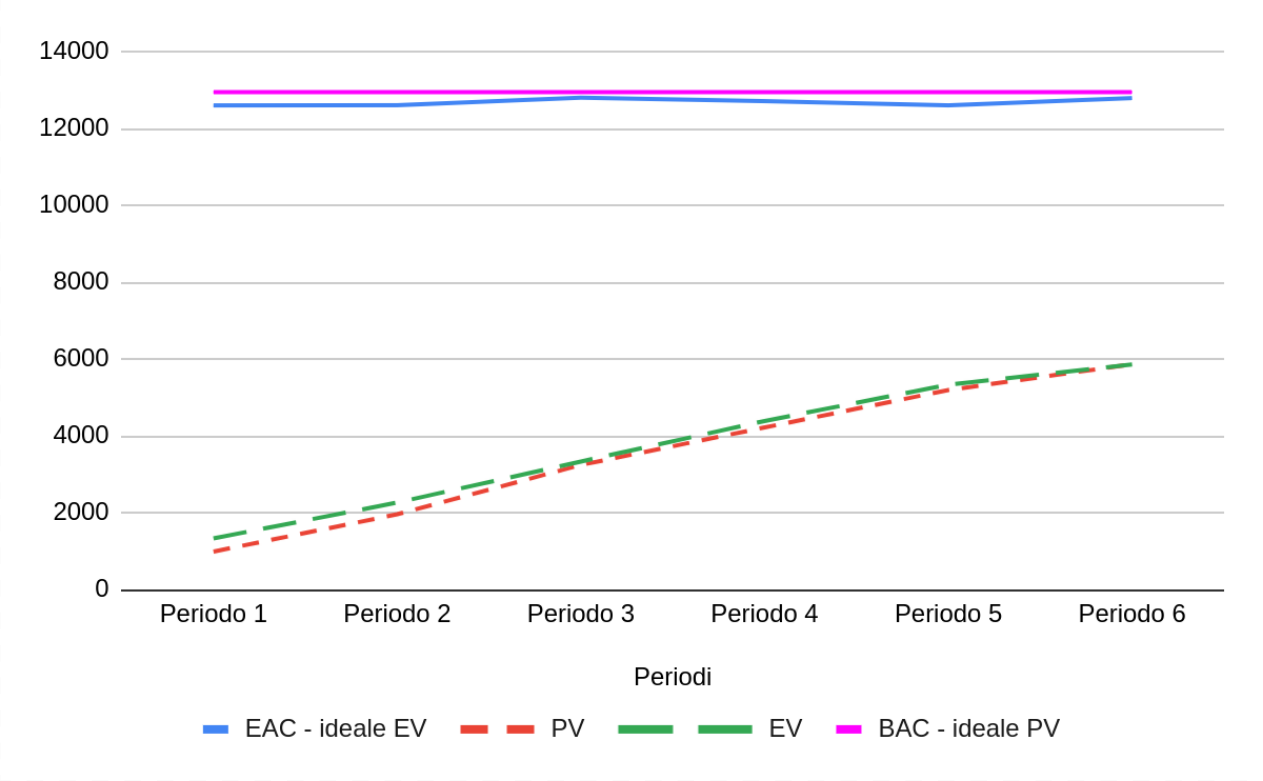
\includegraphics[width=0.9\linewidth]{EV-PV.png}
  \caption{Grafico a linee delle metriche EV$_G$ e PV$_G$}
  \label{fig:EV-PVchart}
\end{figure}

\textbf{RTB}: Il grafico mostra la curva del valore guadagnato (Earned Value), e la curva del valore pianificato (Planned Value). Come si può notare osservando la 
figura le due curve sono molto vicine, questo indica che il lavoro effettivamente svolto è conforme alla pianificazione; e nello specifico quella dell'EV è sempre 
leggermente superiore a quella del PV$_G$. Ciò indica che il progetto$_G$ sta producendo un valore maggiore rispetto a quanto pianificato, e quindi che il lavoro svolto 
è leggermente al di sopra delle aspettative.


\subsubsection{MPC03 - Actual Cost (AC) \& MPC02 - Estimate to Complete (ETC)}

\begin{figure}[H]
  \centering
  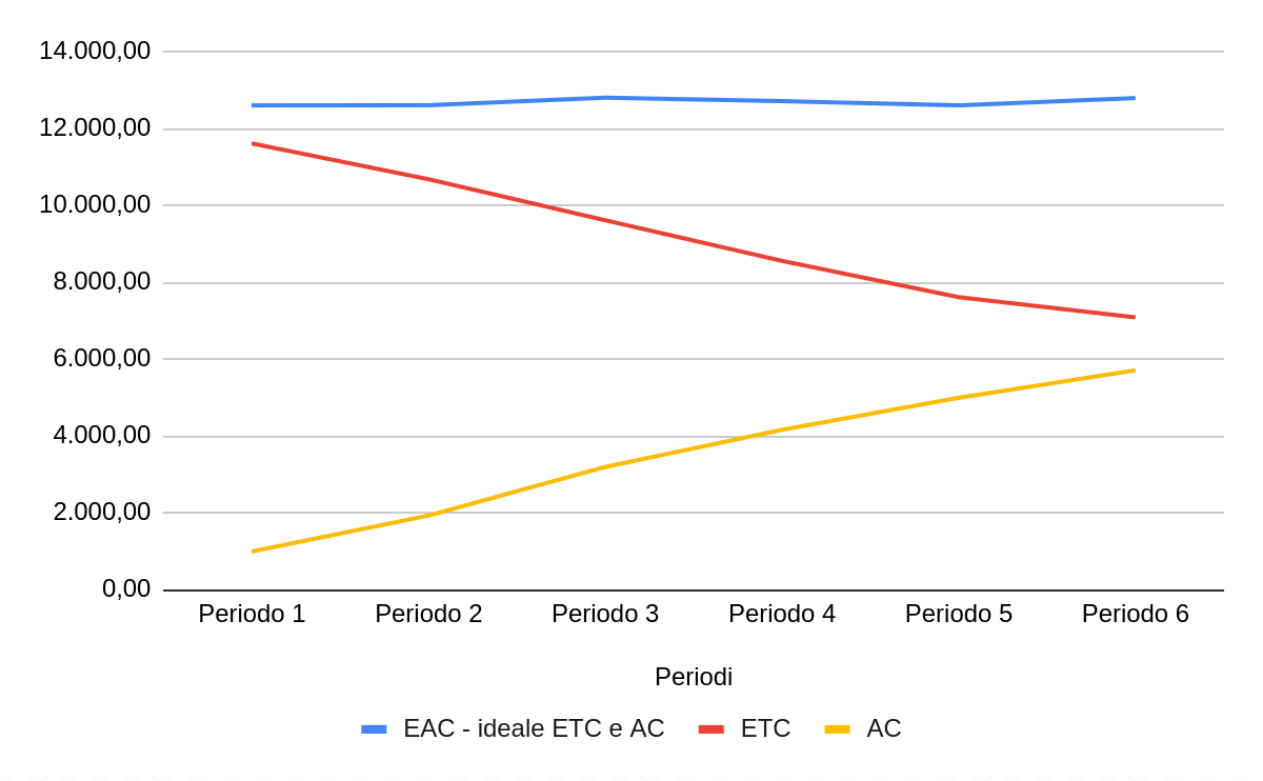
\includegraphics[width=0.9\linewidth]{AC-ETC.png}
  \caption{Grafico a linee delle metriche AC$_G$ e ETC$_G$}
  \label{fig:AC-ETCchart}
\end{figure}

\textbf{RTB}: Il grafico rappresenta l'Actual Cost (AC), ovvero i costi sostenuti per portare il progetto$_G$ al suo stato corrente, e l'Estimate to Complete (ETC), 
cioè la stima del costo rimanente da sostenere per completare il progetto$_G$ per ogni periodo di misurazione (termine sprint$_G$). Entrambe le metriche hanno valore ideale
inferiore all'EAC, che viene rispettato in ogni iterazione.\\
Ovviamente l'ETC tende a diminuire al progredire del progetto$_G$ poiché questo si avvicina alla sua conclusione, mentre l'AC mostra una crescita proporzionale e inversa 
rispetto all'ETC, in linea con le aspettative economiche del progetto$_G$.

\subsubsection{MPC08 - Cost Performance Index (CPI)}

\begin{figure}[H]
  \centering
  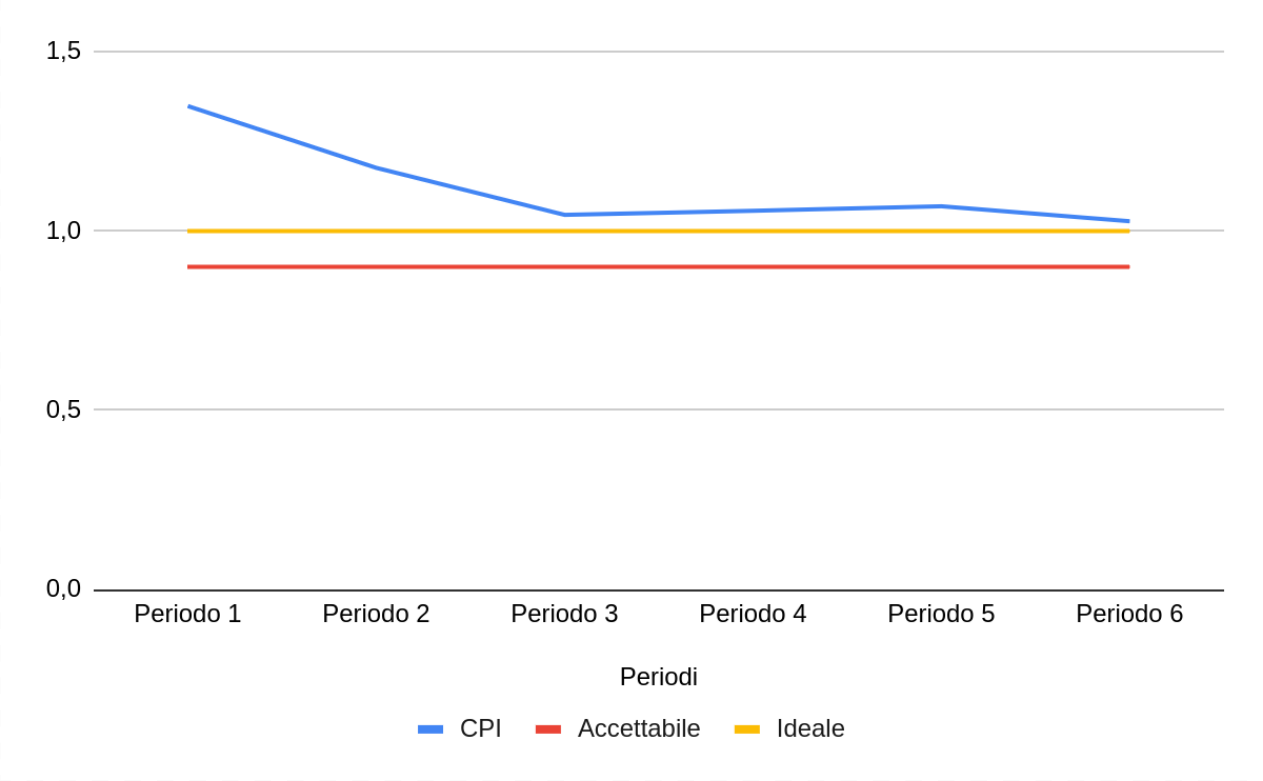
\includegraphics[width=0.9\linewidth]{CPI.png}
  \caption{Grafico a linee della metrica CPI$_G$}
  \label{fig:CPIchart}
\end{figure}

\textbf{RTB}: Il Cost Performance Index (CPI) è una metrica che indica quanti obiettivi sono stati raggiunti rispetto alle spese sostenute in un certo momento del
progetto$_G$. La metrica è data dal rapporto fra il valore guadagnato (EV) e i costi sostenuti (AC), e infatti il suo valore ideale deve essere maggiore o pari a 1.
Il valore accettabile invece è stato scelto essere maggiore o uguale a 0.9.\\
Il grafico mostra che il CPI$_G$ ha avuto valore strettamente maggiore di 1 per tutto il progetto$_G$, assestandosi fra il terzo e il sesto sprint$_G$ a un valore pari a circa 1.06.
Questo indica che il progetto$_G$ ha prodotto un valore maggiore rispetto ai costi sostenuti.


% originariamente qui c'era una sottosezione in più di Pianificazione, che non appare però negli Obiettivi Metrici di qualità (sopra):
% \subsection{Qualità di processo$_G$ - Pianificazione}
% si può rimettere aggiungendo però pianificazione anche nei Obiettivi Metrici di qualità, e volendo inserendo in pianificazione anche la metrica proposta sotto a questa:
\subsubsection{MPC07 - Cost Variance (CV) \& MPC06 - Schedule Variance (SV)}

\begin{figure}[H]
  \centering
  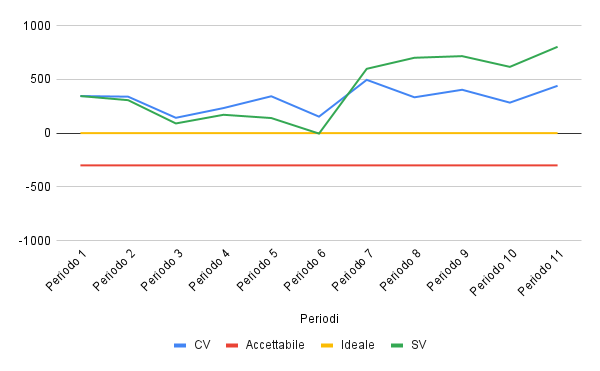
\includegraphics[width=0.9\linewidth]{CV-SV.png}
  \caption{Grafico a linee delle metriche CV$_G$ e SV$_G$}
  \label{fig:CV-SVchart}
\end{figure}

\textbf{RTB}: Il grafico mostra l'andamento  della Cost Variance (CV) e della Schedule Variance (SV), che rappresentano rispettivamente: 
la differenza tra il valore guadagnato (EV) e i costi sostenuti (AC) e la differenza tra il valore guadagnato (EV) e il valore pianificato (PV).\\
La CV$_G$ resta sempre positiva per l'intera durata del progetto$_G$ fino al sesto sprint$_G$, e ciò indica che le spese effettuate sono inferiori rispetto al valore prodotto
dal team nel corso della prima parte del progetto$_G$.\\
La SV$_G$ mostra un andamento positivo fino al quinto sprint$_G$, e ciò indica che il gruppo ha saputo produrre un valore maggiore di quanto
pianificato nel corso delle iterazioni effettuate. Invece per il sesto sprint$_G$ la SV$_G$ è andata ad un valore non positivo.\\
% Possibile aggiunta di una metrica PV$_G$ - AC$_G$ per mostrare gli errori di pianificazione nei preventivi. Bisognerebbe però aggiungere questa metrica anche nelle NdP


\subsection{Qualità di processo$_G$ - Sviluppo}
% da modificare formula in NdP seguendo formula indicata sugli spreadsheets
\subsubsection{MPC10 - Requirements Stability Index (RSI)}  

\begin{figure}[H]
  \centering
  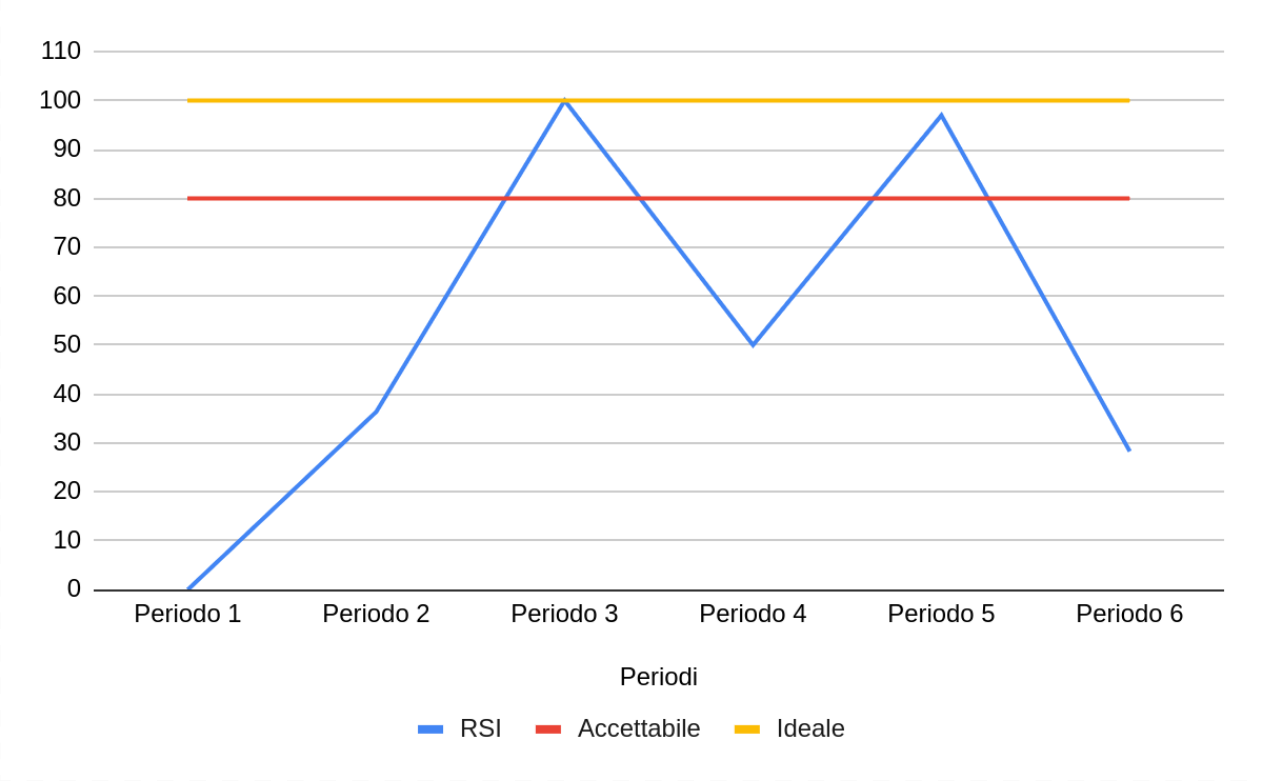
\includegraphics[width=0.9\linewidth]{RSI.png}
  \caption{Grafico a linee della metrica RSI$_G$}
  \label{fig:RSIchart}
\end{figure}

\textbf{RTB}: La metrica RSI$_G$ rappresenta un indice di stabilità dei requisiti individuati nel corso del progetto$_G$. Questo indice è in percentuale e assume valore tanto più alto 
quanto maggiore è la stabilità dei requisiti. In altre parole, il valore è alto se pochi requisiti sono cambiati rispetto all'ultima misurazione, mentre è basso se molti requisiti sono
stati modificati, aggiunti o rimossi rispetto all'ultima misurazione.\\
Come si può evincere dal grafico, l'RSI è partito da valore nullo (in maniera coerente rispetto alla formula usata per il calcolo di tale metrica, poiché nel primo sprint$_G$ 
sono stati definiti i primi requisiti); crescendo nella seconda iterazione (mentre il primo tentativo di identificazione dei requisiti era ancora in corso); e ha poi mostrato 
un andamento altalenante, con picchi di stabilità nel terzo e quinto periodo e cali significativi (inferiori al valore accettabile) in corrispondenza della terza e sesta iterazione. In entrambi questi 
casi il valore basso è seguito a significative modifiche dei requisiti, successive a degli incontri di chiarimento organizzati con il professor Cardin, che  hanno 
evidenziato degli errori nell'approccio del gruppo all'analisi dei requisiti.\\
Complessivamente il gruppo si aspetta una maggiore stabilità in futuro, in caso di un buon esito della revisione RTB$_G$, mentre potrebbero essere necessari ulteriori
significativi cambiamenti in caso di esito negativo.\\


\subsection{Qualità di processo$_G$ - Gestione dei processi}
\subsubsection{MPC16 - Rischi non previsti}

\begin{figure}[H]
  \centering
  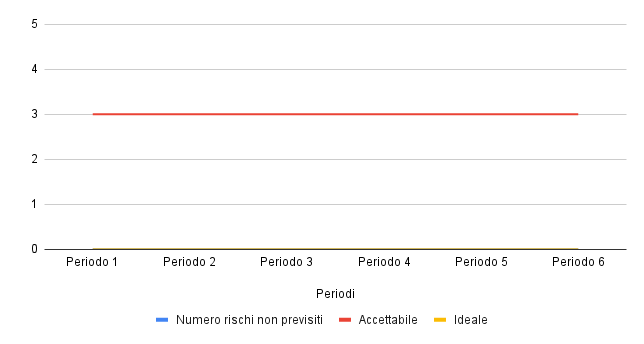
\includegraphics[width=0.9\linewidth]{RNP.png}
  \caption{Grafico a linee della metrica "Rischi non previsti"}
  \label{fig:RNPchart}
\end{figure}

% da rivedere forse. Non so se davvero possiamo dire di non averne incontrati
\textbf{RTB}: Nel corso del progetto$_G$ il team ha senz'altro avuto modo di affrontare svariati dei rischi emersi durante l'analisi dei rischi, tuttavia non sono stati
riscontrati rischi non previsti nel corso dei primi sei periodi del progetto$_G$.


\subsubsection{MPC17 - Efficienza$_G$ temporale (ET)}

\begin{figure}[H]
  \centering
  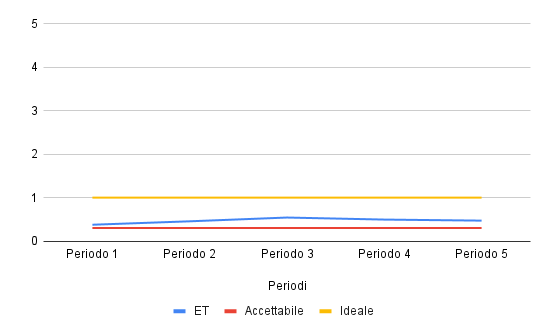
\includegraphics[width=0.9\linewidth]{ET.png}
  \caption{Grafico a linee della metrica ET}
  \label{fig:ETchart}
\end{figure}

% da modificare NdP aggiungendo il fatto che le ore produttive e totali si riferiscono al singolo sprint$_G$ e non all'interezza del progetto$_G$
\textbf{RTB}: La metrica di efficienza$_G$ temporale è data dal rapporto fra il numero di ore produttive e totali per ogni sprint$_G$, e indica quante delle ore dedicate al progetto$_G$
sono state effettivamente usate per la produzione di materiale (software o di altra natura), rispetto alle ore effettivamente consumate dai membri del gruppo. Le ore produttive sono state accuratamente rendicontate per l'intera durata del progetto$_G$, mentre quelle totali (che includono anche le produttive), sono state misurate in
maniera più precisa possibile, ma senza pretese di assoluta esattezza, per via della natura di queste ultime.\\
Dal grafico emerge che la ET si mantiene, per l'intera durata delle prime sei iterazioni del progetto$_G$, poco al di sopra del valore minimo accettabile (pari a 0.2), ma al di 
sotto del valore ideale (pari o superiore a 1.0).\\


\subsection{Qualità di processo$_G$ - Documentazione$_G$}
\subsubsection{MPC01 - Errori ortografici}

\begin{figure}[H]
  \centering
  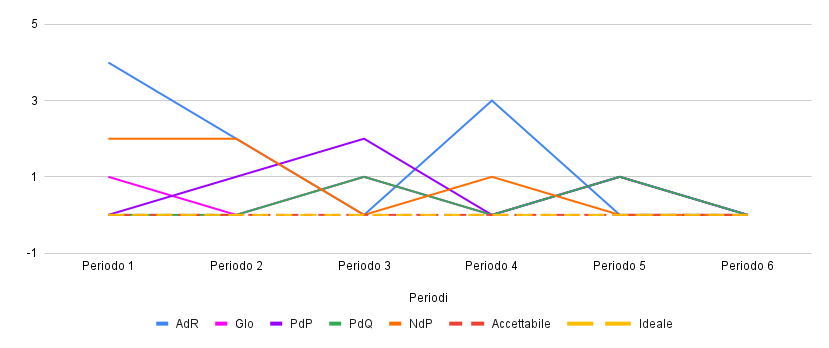
\includegraphics[width=0.9\linewidth]{EO.png}
  \caption{Grafico a linee della metrica "Errori ortografici"}
  \label{fig:EOchart}
\end{figure}

\textbf{RTB}: La metrica rappresenta un indice della qualità della documentazione$_G$ e fa riferimento al numero di errori ortografici individuati in fase di verifica 
dei documenti prodotti.\\
Sebbene il valore ideale non sia mai rispettato nel corso dei primi 5 sprint$_G$ per tutta la documentazione$_G$, è bene evidenziare che il team ha mantenuto comunque dei valori bassi, che hanno 
presentato dei prevedibili aumenti in fasi di grande produzione di documentazione$_G$. L'obiettivo del gruppo è comunque stato quello di consegnare al termine del sesto periodo
dei documenti privi di errori ortografici, e ciò è stato raggiunto, dato che almeno da parte nostra non ne sono stati individuati.\\


\subsubsection{MPC11 - Indice Gulpease}

\begin{figure}[H]
  \centering
  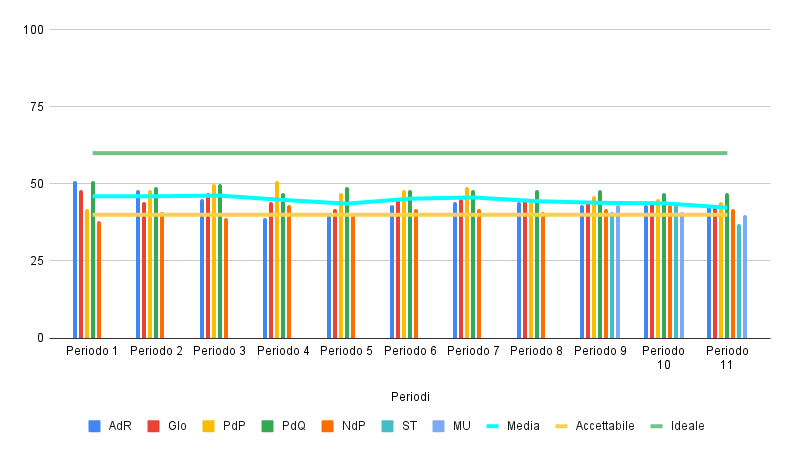
\includegraphics[width=0.9\linewidth]{gulpease.png}
  \caption{Grafico a linee della metrica "indice di Gulpease"}
  \label{fig:gulpease_chart}
\end{figure}

\textbf{RTB}: Emerge da un'analisi del grafico che il valore di accettazione dell'indice di Gulpease (valore ideale $geq$ 60; valore accettabile $geq$ 40), è stato quasi sempre rispettato in tutti i documenti
redatti per cui si è scelto di misurarlo; con alcune eccezioni per il documento \textit{Analisi dei Requisiti} (nel quarto periodo), e per il documento \textit{Norme di Progetto$_G$} (nella prima e nella terza iterazione).\\
Appare tuttavia chiaro che il gruppo ha avuto non poche difficoltà a raggiungere il valore ideale per questa metrica, poiché è stata sottovalutata la difficoltà dello 
scrivere documentazione$_G$ chiara e con linguaggio semplice.\\
A questo proposito il gruppo si porrà in futuro l'obiettivo di migliorare il valore di questa metrica, cercando di esprimere i concetti con frasi più brevi e semplici.\\


\subsection{Qualità di processo$_G$ - Gestione della qualità}
\subsubsection{MPC15 - Metriche di qualità soddisfatte}

\begin{figure}[H]
  \centering
  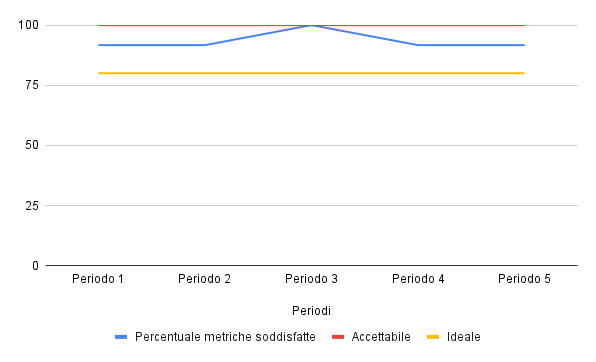
\includegraphics[width=0.9\linewidth]{metricheRispettate.png}
  \caption{Grafico a linee della metrica "metriche di qualità soddisfatte"}
  \label{fig:metricheRispettate_chart}
\end{figure}

\textbf{RTB}: Questa metrica rispecchia la capacità del team di rispettare i valori accettabili delle altre metriche misurata nel corso del progetto$_G$. Dall'analisi del suo 
grafico emerge che il gruppo è sempre riuscito a garantire il rispetto di più dell'90\% delle metriche misurate. Ciò è un segnale chiaramente positivo che dimostra
un buon lavoro del gruppo dal punto di vista della gestione della qualità.\\
Detto ciò è però bene notare che il gruppo, in solo uno dei precedenti sei periodi, ha raggiunto il valore ideale (100\%), quindi CI$_G$ sono comunque importanti margini
di miglioramento da perseguire.\\
Un'ultima nota va aggiunta per specificare che il gruppo ha scelto di considerare la metrica relativa all'indice di Gulpease, che si applica a cinque documenti distinti, come 
una metrica unica facendo la media dei cinque valori misurati.\\

%%%%%%%%%%%%%%%%%%%%%%%%%%%%%%%%%%%%%%%%%%%%%%%%%%%%%%%%%%%%%%%%%%%%%%%%%%%%%%%%%%%%%%%%%%%%%%%%%%%%%%%%%%%%%%%%%%%%%%%%%%%%%%%%%%%%%%%%%%%%%%%%%
%% Queste metriche vanno posizionato sotto la sezione finale in cui si decide di metterli (probabilmente rispettivamente in fornitura e sviluppo)
%%%%%%%%%%%%%%%%%%%%%%%%%%%%%%%%%%%%%%%%%%%%%%%%%%%%%%%%%%%%%%%%%%%%%%%%%%%%%%%%%%%%%%%%%%%%%%%%%%%%%%%%%%%%%%%%%%%%%%%%%%%%%%%%%%%%%%%%%%%%%%%%%

%% Questa metrica è il rapporto fra il valore del lavoro effettivamente svolto e il costo sostenuto per realizzarlo
%% Il Cost Performance Index (CPI) è un indice che misura l'efficienza del progetto$_G$. Un valore maggiore di 1 indica
%% che il progetto$_G$ sta utilizzando le risorse in modo efficiente, mentre un valore minore di 1 indica che il progetto$_G$
%% sta utilizzando le risorse in modo inefficiente.
%% CPI$_G$ = EV$_G$ / AC$_G$
% \subsubsection{MPC01 - Cost performance index (CPI)}
% % Inserire grafico
% \textbf{RTB}: Il grafico mostra che il CPI$_G$ è prossimo ad 1 ma con un leggero calo nel periodo 3. Questo è dovuto al fatto che in questo periodo il team ha ricoperto 
% ruoli più onerosi. Questo ha portato a un aumento dei costi e quindi a un calo del CPI$_G$. Questo calo è comunque accettabile e non preoccupante dato che nel periodo 
% 3 dato il calo di lavoro e avendo ricoperto ruoli più economici c'è stato un bilanciamento.

%% Questa metrica la percentuale di requisiti svolti in percentuale di periodo in periodo
%% Questo dovrebbe valutare la stabilità dei requisiti nel tempo
%% Quindi ogni periodo si raggiunge una percentuale di requisiti svolti
%% E alla consegna della baseline$_G$ RTB$_G$ si raggiunge il 100%, poi per la PB$_G$ si raggiunge il 100% di nuovo.
%% Si va ad obbiettivi, o così l'ho interpretato io
% RSI$_G$ = 100 − {[(RA+RC+RR) / TR] * 100}
% RA: numero di requisiti aggiunti nel periodo considerato;
% RC: numero di requisiti cambiati nel periodo considerato;
% RR: numero di requisiti rimossi nel periodo considerato;
% TR: numero totale di requisiti al momento dell’analisi.
% \subsubsection{MPC01 - Requirements stability index (RSI)}
% % Inserire grafico
% \textbf{RTB}: Questo grafico serve a mostrare l'avanzamento del progresso dei requisiti svolti nel tempo, indicando anche la stabilità nel progresso dei requisiti 
% in percentuale. Inizialmente ovviamente nel primo periodo era a 0. La maggior parte dei progressi sono stati fatti nel 3 periodo con l'analisi dei requisiti e le norme$_G$ 
% di progetto$_G$ e nel 5 periodo con la finalizzazione della documentazione$_G$ citata precedentemente e il completamento del PoC$_G$. Il 4 periodo ha segnato un calo dovuto alle 
% festività natalizie, mentre il 6 periodo ha segnato un calo dovuto alla persante revisione della documentazione$_G$. Questo indice è molto importante per valutare la 
% stabilità dei requisiti nel tempo e per valutare l'efficienza del team nel soddisfare i requisiti.

% Le due sezioni sottostanti saranno da completare per la PB$_G$
% \subsection{Qualità di processo$_G$ - analisi-dei-requisiti$_G$}
% \subsection{Qualità di processo$_G$ - verifica}

%% CI$_G$ sarebbero altre metriche come il code smell e la densità di errori ma non le ho ritenute utili o particolarmente interessanti

\end{justify}
\end{document}
